
\section{总结与展望}

\subsection{本文工作内容总结}
\subsubsection{库位检测系统代码的移植}
和所有的代码移植一样,库位检测系统的代码在移植时也遇到了一些问题。
表 \ref{tab:porting} 给出了移植时遇到的问题与解决方案。

\begin{table}[!hbt]
\centering
\caption{移植问题的解决} \label{tab:porting}
\renewcommand{\arraystretch}{2.62}
%\footnotesize
\begin{tabular}{llll}
\hline 原平台 & 目标平台 & 问题 & 解决方法 \\ \hline
Windows & Ubuntu & MATLAB语言无法直接运行 & \makecell[l]{使用MATLAB自带的代码转换器 \\ 转换为不依赖MATLAB的C/C++代码} \\
Windows & Ubuntu & MATLAB专有I/O库无法调用 & \makecell[l]{使用MATLAB官方的Linux版本库 \\ 或寻找开源的Mat文件读写库} \\
Ubuntu & RCar & \makecell[l]{MATLAB官方的Linux库 \\ 不支持ARM架构} & 切实寻找开源的MATLAB文件读写库 \\
Ubuntu & RCar & PC机与目标机的CPU架构不同 & \makecell[l]{使用RCar专用的交叉编译器 \\ 编译所有源码和相关库} \\
\hline
\end{tabular}
\end{table}

对于因为闭源MATLAB的库导致的问题,解决方案有两种。一种是修改程序,去除对这个库的引用;一种是寻找库的替代品。
环视生成与识别算法会输入训练集,而这个训练集会保存在MATLAB的工作区文件内,即Mat格式。所以对这个库的引用是不能去除的。
虽然通过MATLAB将Mat文件转换为其他形式也是一种方案,但这样做会导致大量的重构,因此只能列为最终的备用方案。

所幸开源的MatIO库 \cite{matio} 很好地提供了MATLAB专用的Mat格式文件的读写。
当然,这个库也定义了一些自定义的接口,与MATLAB的库不同,所以还要写一个API转换代码。
仔细阅读了MatIO库的文档和MATLAB的SDK文档,对比了二者各API功能的区别之后,
就可以完成形如图 \ref{fig:fake} 的API转换代码,从而方便后续的移植操作。

\begin{figure}[!hbt]
\centering
\begin{lstlisting}
mxArray* matGetVariable (MATFile* pMF, const char* name)
{
    // mat_t 与 matvar_t 来自库 MatIO
    mat_t* mf = reinterpret_cast<mat_t*> (pMF);
    matvar_t* content = Mat_VarRead (mf, name);

    // mxArray 与 MATFile 来自 MATLAB 的定义
    return reinterpret_cast<mxArray*> (content);
}
\end{lstlisting}
\caption{API转换代码中一例:数据读取} \label{fig:fake}
\end{figure}


\subsubsection{嵌入式平台上的性能分析}
RCar平台的官方提供了PowerVR套件,其中包含一个系统监视器,即PowerVR Tune \cite{pvrsdk}。
此软件在RCar平静状态下的运行界面如图 \ref{fig:pvrtune} 所示。

\newsavebox{\pvrtune}
\sbox{\pvrtune}{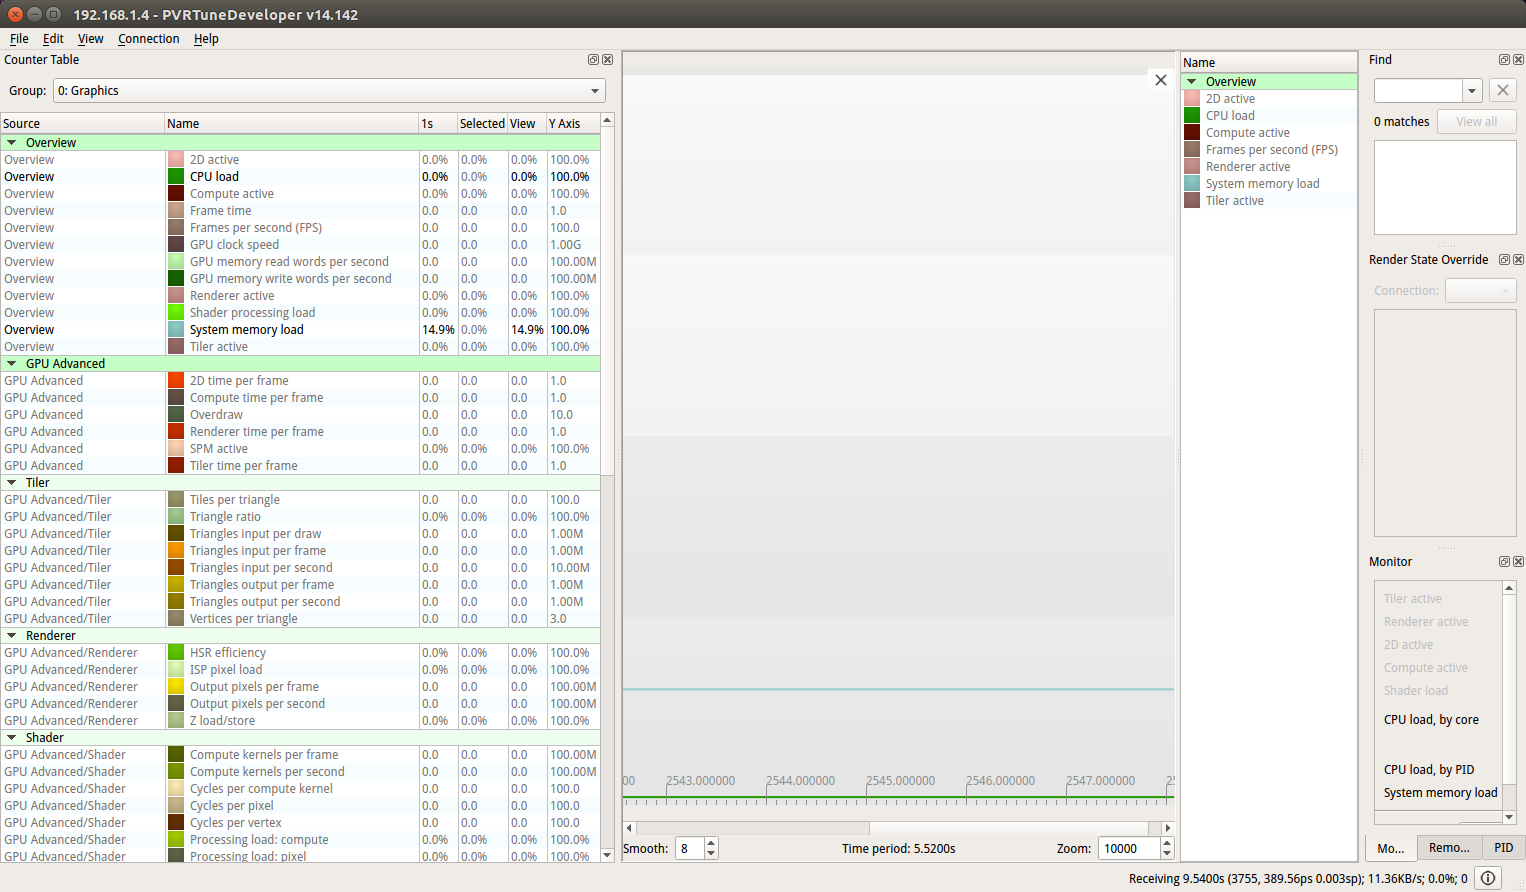
\includegraphics[width=12cm]{image/pvrtune.png}}
\begin{figure}[!hbt]
\centering
\usebox{\pvrtune}
\caption{PowerVR Tune运行截图} \label{fig:pvrtune}
\end{figure}

这个工具分为客户端与服务端。将PC和RCar连接在同一个子网中,通过sftp将服务端上传到RCar上并执行,
再于PC端启动客户端,即可察看RCar上的资源利用情况。

\newsavebox{\pvrtunegpu}
\sbox{\pvrtunegpu}{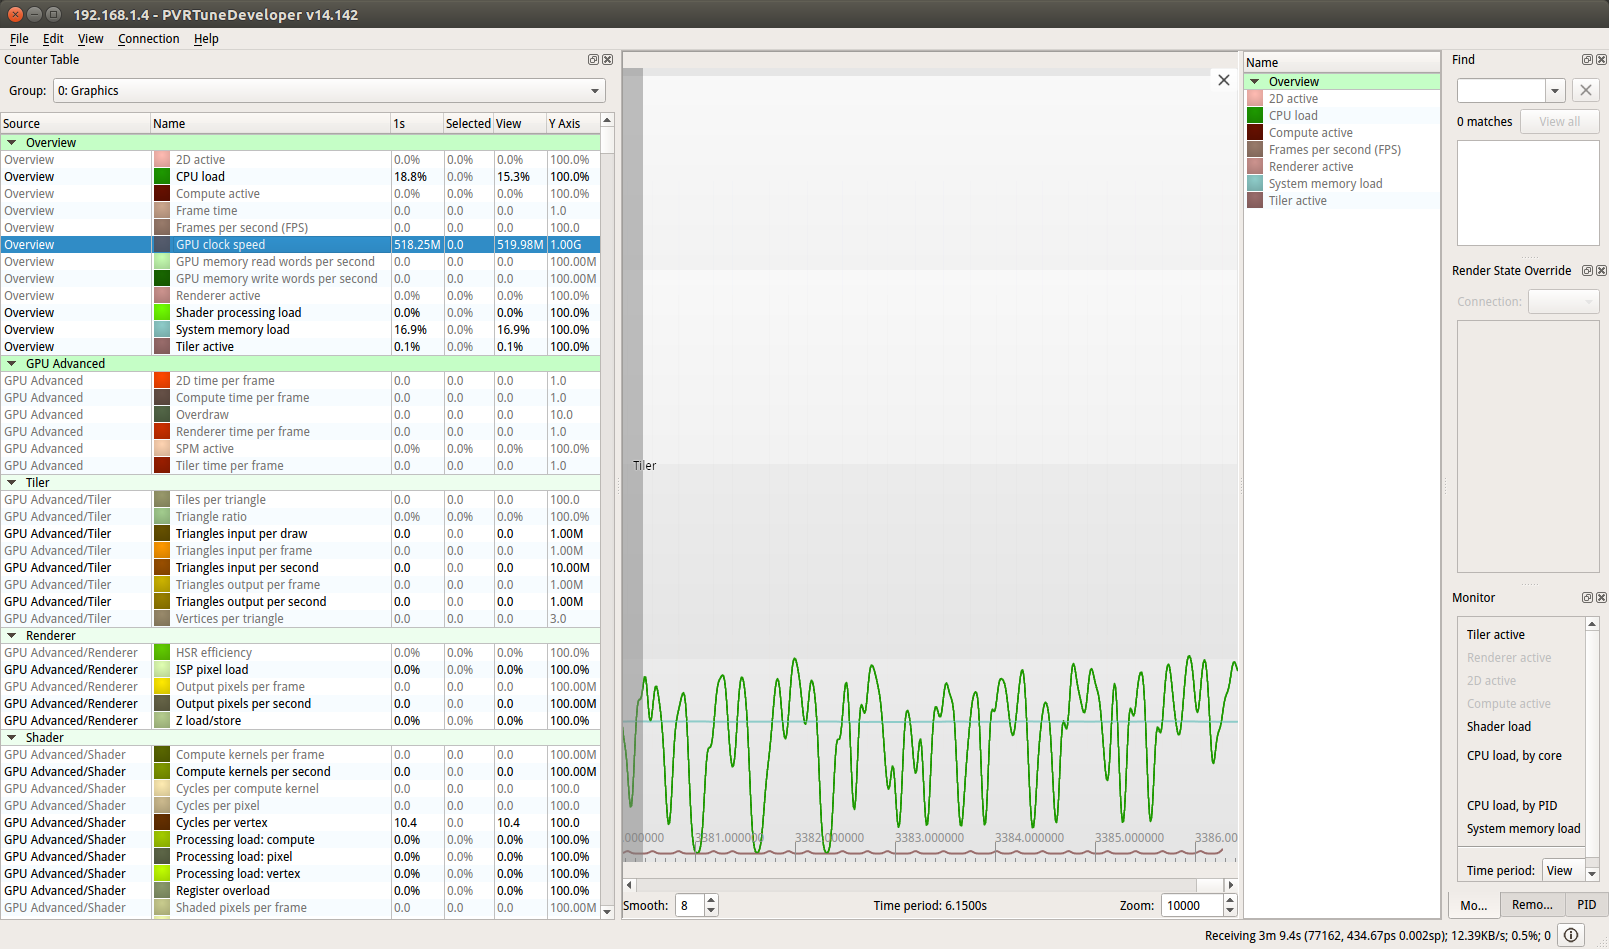
\includegraphics[width=12cm]{image/pvrtunegpu.png}}
\begin{figure}[!hbt]
\centering
\usebox{\pvrtunegpu}
\caption{PowerVR Tune运行截图:占用GPU时} \label{fig:pvrtunegpu}
\end{figure}

如果有的程序正在占用GPU,则PowerVR Tune的界面会如图 \ref{fig:pvrtunegpu} 一样变化。
通过此软件,可以方便地查看程序的资源利用率,以便分析程序在RCar平台上的性能。

此外,PowerVR套件还提供了着色语言编辑器,它为不同版本的着色语言提供了语法检查、代码高亮和预编译功能。
通过这个着色语言编辑器,用户可以方便地写出语法正确的着色语言,集成到项目代码中。为GPU开发和基于GPU的优化提供了方便。

\subsubsection{数据流的生成}
要优化程序,就要得到程序内数据之前的依赖关系,所以需要生成它的数据流图。

对于C/C++两种语言来说,数据流的研究也比其他托管类型的语言更加灵活。
也因此让相关课题的研究有较大的难度。

从上向下看,C/C++语言语法复杂,基于源代码的数据流与控制流分析,需要编写语法解析器。
而这样的语法解析器是难以驾驭的,带来的问题甚至会比数据流与控制流分析本身更多。

从下向上看,尽管控制流的生成甚至可以借助可执行文件的符号文件与反汇编来生成,但数据流却很难这样做。
通过符号文件和反汇编分析数据流时,还要结合源代码重新为寄存器命名,而寄存器数量有限,会被高度重复利用,
再加上汇编代码结构的复杂性,基于汇编的数据流分析是非常困难的任务。

这也就越发体现了LLVM平台的便捷,它从中间出发,利用时空上相互独立的寄存器和简洁高效的LLVM语言表示,
即充分表达了C/C++语言的语义,又屏蔽了底层汇编代码的复杂性。因而成为了十分优秀的代码分析与代码平台。

\subsubsection{数据、控制流向随机Petri网的转化}
数据流可以转换出来,也可以打印出来。但还有一个需求是可以修改数据流。

分析数据流,对它进行修改,然后将修改反馈到源代码中。
修改后的源代码生成新的数据流,再进行分析和优化。如此循环可以不断地让代码更加高效。

但是单一的数据流图是难以在PC上修改的,所以要借助相关的工具。
这时就引入随机Petri网和它的编辑器PIPE5。
将数据流图转换成随机Petri网后,可让研究更加方便。
而许多随机Petri网的编辑器也帮用户更能专注于流程图优化本身。


\subsection{工作内容的不足之处}
\subsubsection{C/C++语言的障碍}
C语言比其他语言更接近低级语言,C++语言也存在如同C语言一样更接近低级语言的特性。
两种语言的编译目标多是生成本地代码(Native Code)。

低级语言非常复杂,接近低级语言的C/C++也比各种托管的语言体现了一定的复杂性。
所以研究它们总是会遇到许多形形色色的障碍,以至于许多想法难以考虑周全。
在这样充满坎坷的领域里做相关研究,要找到一个平衡点,忽视一些对研究影响不深的问题。

\subsubsection{数学上的证明}
从数据流与控制流图向随机Petri网转化,应当证明算法的有效性。
所以要通过数学上的方法研究两种图的关系,并证明这些关系。
限于笔者水平,本文无法给出数学上的证明,这也是本文的一个不足之处。




\subsection{工作结果的展望}

\subsubsection{随机Petri网形式的数据流分析}
得到了代表程序数据流程的随机Petri网后就可以对它进行分析和修改了。
在分析时要找到数据间的依赖关系,找出程序各个流程之间的关系。
重点是找出哪些数据与流程可以同时进行而不会互相干扰。

找到这些后可以设计相关的优化方案。
优化方案的设计还要考虑到平台的软硬件限制,如多线程调度的开销、编译器的支持、被优化算法本身的限制等。
而这又是一个新的课题。

\subsubsection{程序的并行化重构}
基于随机Petri网的分析的结果和相关的优化方案,可以对程序进行重构,以实现程序中算法的并行处理。
多线程处理的技术有UNIX系统经典的pthread标准,也有较新的编译器支持的OpenMP标准。
根据平台上库的支持与平台的交叉编译器的支持,可灵活选择相关方案进行代码重构。

\subsubsection{嵌入式平台基于GPGPU的算法优化}
本文所举的例子平台RCar支持OpenGL ES 3.0,这个版本已经初步支持通用计算(GPGPU)。
但它并没有显式支持通用计算功能,不存在OpenGL ES 3.1开始支持的计算着色器(Compute Shader),
所以要在3.0版本上做通用计算还需要一定的技巧。

例如,利用游戏开发者们在3.0版本上使用的制作粒子效果时使用的技术,
即顶点着色器(Vertex Shader)与导出其计算结果时使用的变换反馈(Transform Feedback)两个功能,
就可完成通用计算的算法。虽然略显复杂,但限于平台支持的功能,这已经是一个很好的结果。

\subsubsection{基于随机Petri网的自动化优化设计}
更为高级而复杂的课题是基于随机Petri网的自动化优化设计。
它要求实现一个软件,分析随机Petri网结构,从中自动找到可以并行化的部分,并为用户提供优化建议。

自动化处理的好处是显然的,它可以进一步简化让程序的并行化优化的分析过程,
同时又能处理大批量的数据。用户通过大量的结果可以给出更为上层的优化方案,让程序的并行化更加简便。
